% ltex: language=it
\chapter{Studio di Fattibilità}\label{chap:studio_di_fattibilita} % (fold)
La necessità di effettuare uno studio di fattibilità nasce dal fatto che si è individuato un possibile progetto, che per dimensione economica, complessità dell'intervento, incertezza sui requisiti, presenza di possibili alternative, richiede un approfondimento prima che possa essere avviata la realizzazione, pena un elevato rischio di insuccesso.
\begin{quote}
    L'obiettivo di uno studio di fattibilità non è quindi quello di individuare potenziali progetti, bensì quello di dare concretezza a un progetto pre-identificato, fornendo tutti gli elementi per l'avvio della fase realizzativa
\end{quote}
Esplicitare le condizioni che rendono conveniente l'effettuazione di progetti per la realizzazione di sistemi informativi automatizzati e l'erogazione di servizi informatici.
In particolare è importante definire esattamente i benefici attesi del progetto, stimare i costi di impianto e di esercizi individuando e valutando i rischi del progetto.
\\
Dare concretezza all'ipotesi progettuale delineando il processo di passaggio dallo stato attuale a quello finale corrispondente alle attese.
In particolare è necessario verificare l'esistenza di un'adeguata soluzione tecnico-organizzativa situata all'interno di vincoli economici e temporali dai anche attraverso il confronto tra soluzioni diverse e la scelta tra essi sulla base di criteri espliciti e predefiniti.
\emptyln{}
Sebbene il contenuto di uno studio di fattibilità vari fortemente in base alla natura del progetto, è possibile delineare la seguente struttura di riferimento:
\begin{itemize}
    \item Analisi della situazione attuale;
    \item Progetti di massima;
    \item Analisi dei rischi;
    \item Il progetto proposto;
    \item Analisi costi benefici;
    \item Raccomandazioni per le fasi realizzative;
\end{itemize}
\begin{note}[Valutazione delle alternative]
    Lo studio di fattibilità presuppone la valutazione di diverse alternative progettuali.
    È però indispensabile delineare con esattezza i margini decisionali di competenza dello studio di fattibilità al fine di non stravolgerne gli obiettivi.
    \begin{center}
        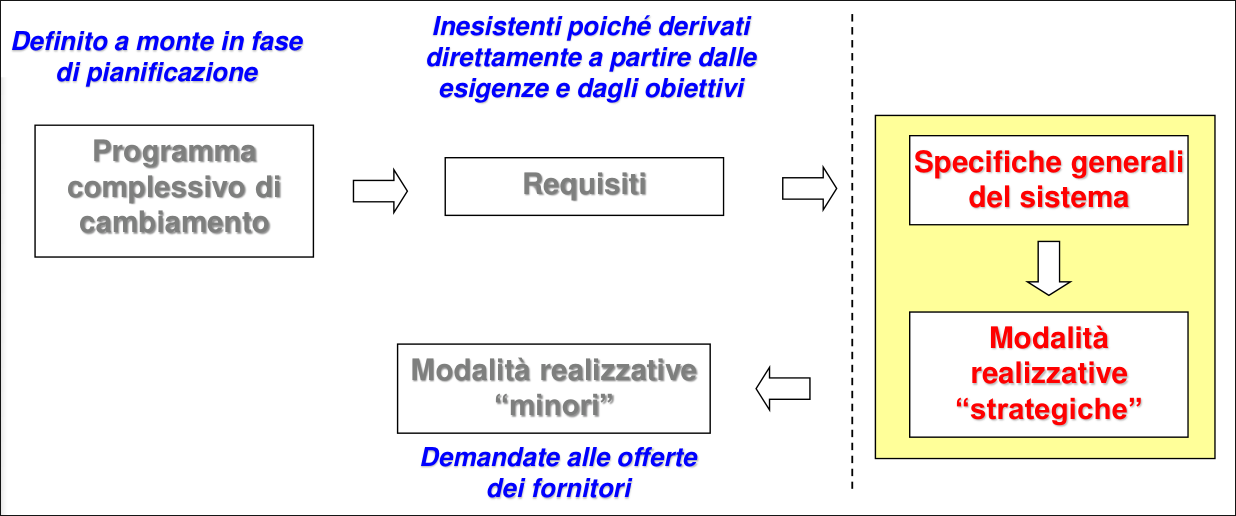
\includegraphics[width=.8\textwidth]{assets/fatt-altern-visual.png}
    \end{center}
\end{note}
%
\section{Analisi della Situazione attuale}\label{sec:ftt_analisi_della_situazione_attuale} % (fold)
L'analisi della situazione attuale evidenzia le caratteristiche del sistema informativo su cui deve essere realizzato il progetto relativo allo studio di fattibilità e si articola sui seguenti punti:
\begin{itemize}
    \item il contesto dello studio: serve a inquadrare il progetto analizzato nel quadro della strategia di sviluppo dei \hyperref[sub:il_sistema_informativo]{SI}
        \begin{itemize}
            \item ripresa della visione strategica in termini di servizi, organizzazione, tecnologia;
            \item ripresa dei principali passaggi che hanno portato all'individuazione del progetto;
            \item collocazione del progetto all'interno del piano d'informazione;
        \end{itemize}
    \item descrizione delle problematiche: illustra i problemi o le opportunità da cui scaturisce il progetto, indicandone la rilevanza e stabilendone esattamente i confini
        \begin{itemize}
            \item descrizione e rilevanza della problematica;
            \item esigenze da soddisfare (rispetto a utenti interni ed esterni);
        \end{itemize}
    \item descrizione della situazione attuale del \hyperref[sub:il_sistema_informativo]{SI}: individuazione e rappresentazione dei processi e dei sistemi informatici coinvolti nell'area di intervento
        \begin{itemize}
            \item individuazione e rappresentazione dei processi coinvolti;
            \item individuazione e rappresentazione dei flussi informativi;
            \item individuazione e rappresentazione della struttura organizzativa e dell'utenza coinvolta;
            \item attuale livello di automazione;
        \end{itemize}
    \item analisi e diagnosi della situazione attuale: illustra i risultati dell'attività di esame e valutazione critica dei processi impattati dal progetto, risultati finalizzati alla individuazione e quantificazione degli obiettivi di progetto:
        \begin{itemize}
            \item individuazione dei fenomeni che costituiscono le cause del problema;
            \item collocazione di tali fenomeni sulle diverse componenti dei processi di servizio;
            \item individuazione di metriche atte a rappresentare fenomeni critici e la loro evoluzione;
            \item misurazione della situazione attuale;
        \end{itemize}
    \item identificazione dei vincoli: identifica e descrive le condizioni di ambiente non modificabili della situazione attuale
        \begin{itemize}
            \item quadro normativo di riferimento;
            \item vincoli temporali e altri vincoli (economici, organizzativi, ...);
        \end{itemize}
    \item definizione degli obiettivi di progetto: gli obiettivi devono essere espressi in forma quantitativa, ossia debbono fare riferimento a costi, tempi e a individuate caratteristiche del prodotto/servizio erogato oltre a essere messe in relazione con i fenomeni individuati come cause dei problemi da cui il progetto ha avuto origine;
\end{itemize}
\begin{note}
    Parte delle informazioni richieste in queste fasi dovrebbero essere già presenti in azienda poiché elaborate durante la fase di pianificazione, è quindi necessario riutilizzarle approfondendole dove necessario
\end{note}
% section Analisi della Situazione attuale (end)
%
\section{Progetti di Massima}\label{sec:ftt_progetti_di_massima} % (fold)
I \textbf{progetti di massima} consistono in una descrizione generale del sistema informativo previsto e comprendono:
\begin{itemize}
    \item \textbf{definizione dei requisiti}, ossia delle condizioni che il sistema deve soddisfare;
    \item \textbf{specificazioni del sistema} ossia una descrizione del sistema proposto in \textbf{termini di proprietà};
    \item l'indicazione delle principali modalità di realizzazione;
\end{itemize}
\begin{quote}[A che livello di dettaglio deve essere realizzato lo studio di fattibilità?]
    Lo studio di fattibilità deve essere realizzato a un livello di dettaglio tale da rispondere ai quesiti per cui è stato richiesto
\end{quote}
Dovrà quindi essere svolto a un \textbf{elevato livello di aggregazione} intendendo che non tutte le componenti del \hyperref[sub:il_sistema_informativo]{SI} dovranno essere completamente scomposte e descritte.
Dovranno essere studiate solo le \textbf{funzionalità principali} e i casi di utilizzo standard.
\begin{note}
    Lo studio potrà riguardare \textbf{solo la porzione più importante} del \hyperref[sub:il_sistema_informativo]{SI} che presenta le principali criticità e su cui incombono i principali dubbi.
    \emptyln{}
    Possono essere proposti diversi progetti di massima le cui caratteristiche verranno valutate durante lo studio di fattibilità.
\end{note}
\begin{description}
    \item[Requisiti della soluzione] Devono essere evidenziate le condizioni essenziali che il sistema proposto deve rispettare:
        \begin{itemize}
            \item dettaglio del processo previsto;
            \item interventi previsti sulle componenti non informatizzate del processo;
            \item necessità di modifica della normativa;
            \item requisiti del sistema informativo da realizzare;
        \end{itemize}
    
    \item[Specifiche generali del sistema] Evidenzia le specifiche di massima del sistema informativo da realizzare, ossia quelle caratteristiche o proprietà  che sono essenziali per rispondere ai requisiti individuati:
        \begin{itemize}
            \item Specifiche Applicative:
                \begin{itemize}
                    \item architettura dei dati (con esame e valutazione delle eventuali alternative);
                    \item architettura applicativa (con esame e valutazione delle eventuali alternative);
                    \item interfaccia utente;
                \end{itemize}
            \item Specifiche Tecnologiche:
                \begin{itemize}
                    \item architettura tecnologica (con esame e valutazione delle eventuali alternative);
                    \item ambiente e strumenti di sviluppo (con esame e valutazione delle eventuali alternative);
                \end{itemize}
        \end{itemize}
    \item[Modalità di realizzazione] Si sviluppa attraverso le seguenti linee guida per definire la fattibilità tecnica, economica e operativa dell'intervento:
        \begin{itemize}
            \item realizzazione o acquisizione (con esame e valutazione delle eventuali alternative);
            \item riuso dei componenti esistenti (con esame e valutazione delle eventuali alternative);
            \item avvio del sistema;
            \item esercizio e manutenzione del sistema;
            \item formazione e assistenza utenti;
        \end{itemize}
\end{description}
% section Progetti di Massima (end)
%
\section{Analisi del Rischio}\label{sec:ftt_analisi_del_rischio} % (fold)
Il \textbf{rischio} connesso a un progetto è dato dall'esistenza di eventi capaci di pregiudicare il buon esito del progetto:
\begin{itemize}
    \item mancata conclusione;
    \item ottenimento di prodotti difettosi;
    \item lievitazione dei costi;
    \item allungamento dei tempi;
    \item difficile integrazione con il restante sistema informativo;
\end{itemize}
\begin{description}
    \item[Individuazione dei fattori di rischio del progetto] Evidenzia i principali fattori di rischio:
        \begin{itemize}
            \item \textbf{complessità}:
                \begin{itemize}
                    \item complessità gestionale;
                    \item dimensione del progetto;
                    \item altri fattori specifici;
                \end{itemize}
            \item \textbf{incertezza}:
                \begin{itemize}
                    \item incertezza sui requisiti;
                    \item innovazione tecnologica;
                \end{itemize}
        \end{itemize}
    
    \item[Definizione del rischio di progetto] Valuta sistematicamente tutti i fattori di rischio individuati e determina la classe di rischio dell'intero progetto.
    Ha l'obiettivo di individuare in maniera precisa i rischi connessi a un progetto.
    \\
    L'esito di tale quantificazione consiste nell'attribuzione alle varie fasi del progetto di un'appropriata \textbf{classe di rischio}.
    \\
    L'esecuzione dell'analisi prevede le seguenti fasi:
        \begin{enumerate}
            \item individuazione di un insieme di fattori di rischio;
            \item per ogni fattore di rischio si definisce un insieme di parametri quantificabili;
            \item per ogni parametro si quantifica il livello di rischio (alto/medio/basso);
        \end{enumerate}
    \item[Modalità di gestione del rischio] Definisce una strategia e un insieme di azioni tese alla riduzione dei rischi e quindi al buon andamento del progetto.
        L'individuazione dei fattori di rischio deve portare alla definizione delle modalità di \textbf{gestione del rischio} ossia degli accorgimenti adottabili per ridurre i rischi del progetto:
        \begin{itemize}
            \item \textbf{individuazione degli elementi critici}: ossia delle fasi che mettono maggiormente a rischio la riuscita dell'intero progetto.
                Tali fasi saranno soggette a un maggior controllo e su di esse andranno concentrate un maggior numero di risorse.
            \item \textbf{segmentazione}: la segmentazione riduce i rischi del processo poiché permette di circoscrivere e controllare meglio i rischi inerenti alla complessità, alla dimensione e all'incertezza;
            \item \textbf{definizione dei punti di controllo}: indicano i momenti in cui valutare lo stato del progetto per verificarne l'andamento in base ai fattori critici ed eventualmente valutare modifiche in corso d'opera;
            \item \textbf{definizione dei punti di accesso}: nel caso si verifichino i problemi legati ai fattori di rischio può essere opportuno interrompere il progetto prima che questo porti a ulteriori danni per l'azienda;
        \end{itemize}
\end{description}
% section Analisi del Rischio (end)
%
\section{Il Progetto proposto}\label{sec:ftt_il_progetto_proposto} % (fold)
Sulla base di quanto indicato nel progetto di massima e tenendo in considerazione i risultati dell'analisi del rischio specifica la soluzione scelta indicando più in dettaglio tempi e modi di realizzazione.
Questa fase si articola su quattro punti:
\begin{description}
    \item[Segmentazione del processo] Si intende la suddivisione di un progetto in moduli ognuno finalizzato al completamento di un sottosistema specifico.
        La modalità di segmentazione dipende dalle scelte realizzative fatte.
        \begin{itemize}
            \item \textbf{realizzazione in soluzione unica}: il \hyperref[sub:il_sistema_informativo]{SI} viene realizzato, e collaudato in un'unica versione, generalmente con una attività continuativa;
            \item \textbf{realizzazione incrementale}: la realizzazione e il collaudo avvengono per parti successive, ciascuna delle quali contiene un sotto insieme delle funzionalità e dei servizi previsti.
                I requisiti previsti sono completamente definiti prima della realizzazione iniziale e non variano nel corso delle successive installazioni;
            \item \textbf{realizzazione evolutiva}: la realizzazione e il collaudo avviene per versioni successive in cui ogni versione può contenere tutte o parte delle funzionalità e dei servizi previsti.
                I requisiti previsti possono essere variati tra due versioni successive in seguito al feedback ottenuto durante le fasi di realizzazione e collaudo;
            \item \textbf{approccio Agile}: fortemente incrementale ed evolutivo.
                L'interazione con l'utente è finalizzata ad acquisire feedback utili al miglioramento in corso d'opera.
                Rispetto alle soluzioni precedenti si prevede esplicitamente nel progetto l'inserimento/rimozione di funzionalità nonché la ri-prioritizzazione delle consegne in base al cliente;
        \end{itemize}
    \item[Riepilogo delle acquisizioni e realizzazioni previste]  Focalizza definitivamente il progetto realizzativo proposto alla luce dei criteri di segmentazione scelti e sintetizza le acquisizioni previste (sistemi di elaborazione, servizi e apparecchiature di rete, software di base e applicativo);
    \item[Modello Organizzativo] Definisce la struttura organizzativa finalizzata alla gestione del progetto e le modalità di interazione fornitore-cliente.
        \begin{itemize}
            \item struttura organizzativa preposta al progetto per il committente:
                \begin{itemize}
                    \item articolazione, figure ``chiave'', compiti e responsabilità e competenze;
                    \item valutazione (di massima) degli impegni richiesti a utenti di business, personale del \hyperref[sub:il_sistema_informativo]{SI};
                \end{itemize}
            \item struttura organizzativa richiesta dal fornitore:
                \begin{multicols}{2}
                    \begin{itemize}
                    \item articolazione, con chiara individuazione del Responsabile di Progetto e, se applicabile, dei diversi Responsabili di Servizio;
                    \item definizione dei compiti e delle responsabilità;
                    \item modalità operative di interazione tra Amministrazione committente e fornitore: classificazione delle forme di interazione previste (riunioni, prodotti e documenti, etc);
                    \end{itemize}
                \end{multicols}
            \item eventuali strumenti e/o sistemi informatici a supporto di dette interazioni: SharePoint, Microsoft Project, ErWin;
        \end{itemize}
    \item[Piano di Progetto] Esplicita la sequenza e le dipendenze tra le principali attività del progetto.
        Esso deve evidenziare la necessità e gli obiettivi di fondo cui la programmazione puntuale delle attività dovrà adeguarsi per rispettare sia le scadenze temporali fissate, sia la coerente disponibilità dei prodotti intermedi necessari al progressivo superamento dell'incertezza e alla definizione di dettaglio dei prodotti finali attesi.
        \begin{itemize}
            \item \textbf{Piano dei rilasci}:
                \begin{itemize}
                    \item requisiti globali;
                    \item specifiche realizzative di fondo;
                    \item specifiche di dettaglio;
                    \item produzione prototipi;
                    \item installazione sistema finale;
                \end{itemize}
            \item \textbf{Punti di controllo};
            \item \textbf{Piano delle attività}:
                \begin{itemize}
                    \item \textbf{\acf{wbs}};
                    \item Diagramma di Gantt di massima;
                    \item Diagramma di Pert di massima;
                \end{itemize}
        \end{itemize}
\end{description}
%
\subsection{Work Breakdown Structure}\label{sub:ftt_wbs} % (fold)
La \acf{wbs} costituisce una rappresentazione del progetto,
% subsection Work Breakdown Structure (end)
% section Il Progetto proposto (end)
% chapter Studio di Fattibilità (end)
